\documentclass[../main.tex]{subfiles}
\begin{document}
	\begin{defin}
		Кв. ф. $f$ называется приведенной к \underline{каноническому виду}, если все $a_{ij} = 0 \; \; \; i \neq j\n 
		A = diag(a_{11} \ldots a_{nn})$\n 
		Число $a_{ii}>0$ называется \underline{положительным индексом} инерции кв. ф.
		\[\sigma^+ (f) = \sigma^+\]
		Число $a_{ii} < 0$ называется \underline{отрицательным индексом} инерции кв. ф.
		\[\sigma^- (f) = \sigma^-\]
		Число $a_{ii} = 0$ обозначим за $\sigma^0(f) = \sigma^0$\n 
		$\sigma(f) = (\sigma^+, \sigma^-, \sigma^0) $ \underline{сигнатура кв. ф.} ($\sigma^+ - \sigma^-$ тоже сигнатура)\n 
		$rg f = (\sigma^+ + \sigma^-)$ инвариант $\leadsto \sigma^0 = n - rg \ f$ инвариант относительно $Q$. 
	\end{defin}
	\begin{defin}
		Канонический вид кв. ф. $f$ называется \underline{нормальным}, если все ненулевые $a_{ii} = \pm1$\n 
		Очевидно, всегда $\exists Q$ \Space $\underset{x}{\text{канонич}} \overset{Q}{\leadsto} \underset{y}{\text{нормальн}}$. \n 
		$Q = diag(\underset{\text{невырожд}}{q_1 \ldots q_n}) \Space \begin{matrix}
			q_i = \mathlarger{\frac{1}{\sqrt{|a_{ii}|}}} & a_{ii} \neq 0\\
			q_i = 1 & a_{ii} = 0
		\end{matrix}\n 
		x = Q y$\n 
		Канонич. вид $\ldots + \underbrace{a_{ii}}_{>0} x^2_i + \ldots + \underbrace{a_{jj}}_{<0} x_j^2 + \ldots \underset{x_i = \mathlarger{\frac{y_i}{\sqrt{|a_{ii}|}}}}{\leadsto} \ldots + 1 \cdot y^2_i \ldots - y^2_j - \ldots$
	\end{defin}
	\textbf{Основная задача теории кв. форм}: Найти линейное невырожд. преобр. $Q: x = Qy$, т.ч. 
	кв. ф. $f$ будет приведена к канонич. (норм.) виду ($g(y)$)\n 
	Т.е. $\underset{\text{невырожд.}}{\exists \; Q ?} \; \; \; Q^T A Q = \Lambda = diag(\lambda_1 \ldots \lambda_n)  \; \circled{?}$
	\subsection{Методы приведения кв. ф. к канонич. виду}
	\paragraph{I. Ортогональное преобразование:} (канонич. вид симм. м-цы)\ \\
	$x \in \R^n \Space x = Qy \Space y \in \R^n \Space f(x) = x^T A x \Space A = A^T\n 
	A$ -- матрица оператора в о.н.б. (канонич. базис $\R^n$) \n 
	$\underset{\stackrel{\uparrow}{\begin{matrix}
				\text{в исходном}\\
				\text{канон. базис } e
			\end{matrix}}}{x}$ и $\underset{\stackrel{\uparrow}{\begin{matrix}
				\text{в новом}\\
				\text{о.н.б. } \R^n \ e'
			\end{matrix}}}{y}$ координаты в разных базисах. \Space $Q = \underset{\begin{matrix}
			\text{ортогон.}\\\text{т.к. } e, e' \text{ о.н.б.}
	\end{matrix}}{T_{e\rightarrow e'}} (Q^T = Q^{-1})\n 
	Q^{-1} A Q = Q^T A Q = B \Space \underset{\text{кв. ф.} A}{f} \overset{x = Q y}{\leadsto} \underset{\text{кв. ф. } B}{g}$\n 
	$\exists?\; \;  e'$, т.ч. $B = diag(\lambda_1 \ldots \lambda_n) = \Lambda$\n 
	---Да\n
	$A = A^T$ симметр. матр. (матр. самосопр. опер.) $\Rightarrow$ канонич. вид симм. матрицы (см. соотв. следствие) \n
	все с.ч. $\lambda_i$ вещ. и $\exists$ базис из о.н.с.в. $A: \; \; v_1 \ldots v_n \Space Q = (v_1 \ldots v_n) \leadsto \Lambda = diag(\underset{\text{собств. ч.}}{\lambda_1 \ldots \lambda_n})$
	\paragraph{II. Метод Лагранжа (метод выделения полного квадрата)}\
	\begin{mylist}
		\item $\forall i \; a_{ii} = 0 \Rightarrow \exists a_{ij} \neq 0 \; \; i \neq j\n 
		x = Q y \Space \left[\begin{array}{c}
			x_i = y_i + y_j \\
			x_j = y_i - y_j \\
			x_k = y_k \; \; \begin{matrix}
				k \neq i\\
				k \neq j
			\end{matrix}
		\end{array}\right. \Space Q = $\belowbaseline[-70pt]{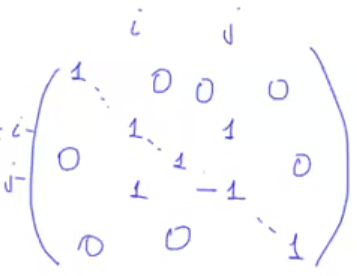
\includegraphics[width=150px]{pic33}} Очевидно, невырожд.\n 
		$f(x) = x^T A x = y^T B y = g(y) = \ldots + \underset{\neq 0}{\overset{b_{ii}}{a_{ij}}} y_i^2 + \ldots \underset{\neq 0}{\overset{b_{jj}}{-a_{ij}}} y_j^2 + \ldots \n 
		a_{ij} x_i x_j = a_{ij} (y^2_i - y^2_j)$
		\item $\exists a_{ii} \neq 0$\\
		Выпишем все слагаемые из $f$, которые соодержат $x_i\n 
		\frac{a_{ii}}{a_{ii}}(\underset{\neq 0}{a_{ii}} x_i^2 + 2 \sum\limits_{\stackrel{j = 1}{j \neq i}}^n a_{ij} x_i x_j) = \frac{1}{a_{ii}}  (\sum\limits_{j=1}^n a_{ij} x_j)^2 - \overset{\text{нет переменной } x_i}{\boxed{\frac{1}{a_{ii}} \sum\limits_{\stackrel{j=1}{j\neq i}}^n x_j^2 a_{ii}^2 - \frac{2}{a_{ii}} \sum\limits_{
					\underset{j\neq i}{\stackrel{1\leq k \leq j \leq n}{k \neq i}}} a_{ik} a_{ij} x_k x_j}}$\n 
		Поместим обратно в форму $f$\n 
		$f(x) = f(x_1 \ldots x_i \ldots x_n) = \frac{1}{a_{ii}}(\sum\limits_{j=1}^n a_{ij} x_j)^2 + \tilde{f} (\underset{\stackrel{\uparrow}{\text{кв. ф. не содержит}}}{x_1 \ldots \hat x_i \ldots x_n})\n 
		Q^{-1}; \Space \left[\begin{array}{c}
			y_i = \sum\limits_{j=1}^n a_{ij} x_j \n 
			y_k = x_k \; \; k \neq i
		\end{array}\right. \Space Q^{-1} = \begin{pmatrix}
			1 & & & & &0\\
			& \ddots\\
			a_{i1} & & a_{ii} & \ldots& & a_{1n}\\
			& & &  1\\
			& & & &\ddots\\
			0 & & & & & 1
		\end{pmatrix} \; \; \; a_{ii} \neq 0$ \n Очевидно, невыр. $\Rightarrow Q$ невыр. $x = Q y$\n 
		Далее повторяем алгоритм для $\hat f$, пока не исчерпаем все переменные.
	\end{mylist}
	\paragraph{III метод Якоби (унитреугольное преобразование)}\ \\ 
	$LU$ разложение матрицы.\n 
	$A = A^T \Space \triangle_k \neq 0 \; \; \; k = 1 \ldots n-1 \; \Rightarrow \begin{matrix}
		\exists! \; U \overset{\text{невырожд.}}{\text{ унитреуг. }}\text{верхн. матр: } A = U^T DU\n 
		\exists! \; L \text{ унитреуг. нижн. матр: } A = LD L^T
	\end{matrix}\n 
	Q = U^{-1}\; \; \;  \underset{=Q^T}{(U^T)^{-1}} A \underset{=Q}{U^{-1}} = D$
	\begin{remark}
		Метод Якоби не является универсальным, т.е. применим не для всех кв. ф., а только для форм, у которых $\triangle_k \neq 0 \; \forall k = 1 \ldots n-1$ (т.е. $rg f \geq n-1$)
	\end{remark}	
	\begin{theorem}[Якоби]
		$A = A^T, \; \triangle_k \neq 0 \; \; k = 1 \ldots n-1\n$
		\begin{minipage}{0.5\textwidth}
			$A = \begin{pmatrix}
			\begin{matrix}
			\begin{matrix}
			\\ a_{11}\\a_{12}\\a_{13}
			\end{matrix} & \begin{matrix}b_2\\
			\boxed{a_{12}}\\a_{22}\\a_{23}
			\end{matrix} & \begin{matrix}b_3\\\boxed{
				\begin{matrix}
				a_{13}\\a_{23}
				\end{matrix}}\\a_{33}
			\end{matrix} & \begin{matrix}
			\ldots\\\ldots\\\ldots
			\end{matrix} & \begin{matrix}b_n\\\boxed{\begin{matrix}
				a_{1n}\\a_{2n}\\a_{3n}
				\end{matrix}}\end{matrix}
			\end{matrix}\\
			\begin{matrix}
			\ldots & \ldots & \ldots & \ldots & \ldots\\
			a_{1n} & a_{2n} & a_{3n} & \ldots & a_{nn}
			\end{matrix}
			\end{pmatrix}$
		\end{minipage}
		\begin{minipage}{0.5\textwidth}
			$\exists!$ унитреуг. верхняя матрица $Q$, т.ч.\n 
			$Q^T A Q = D = diag(\triangle_1 , \frac{\triangle_2}{\triangle_1}, \ldots, \frac{\triangle_n}{\triangle_{n-1}})$
		\end{minipage}\n 
		При этом:\n 
		$Q = \begin{pmatrix}
			\begin{matrix}
				\\1\\0\\0\\\ldots\\0
			\end{matrix} & \begin{matrix}
				q_2\\
				\boxed{q_{12}}\\1\\0\\\ldots\\0
			\end{matrix} & \begin{matrix}
				q_3\\
				\boxed{\begin{matrix}
					q_{13}\\q_{23}
					\end{matrix}}\\1\\\ldots\\0
			\end{matrix} & \begin{matrix}
				\\\ldots\\\ldots\\\ldots\\\ldots\\\ldots
			\end{matrix} & \begin{matrix}
				q_n\\\boxed{\begin{matrix}
						q_{1n}\\q_{2n}\\\ldots\\ q_{n-1\ n}
					\end{matrix}}\\1
			\end{matrix}
		\end{pmatrix}$, где $\boxed{\begin{matrix}
				A_{k-1} q_k = - b_k \\
				k = 2 \ldots n
			\end{matrix}} \; \; (\begin{matrix}
			\triangle_k = |A_k| \neq 0 \; \; k = 1 \ldots n-1\\
			\Rightarrow \text{ все системы имеют един. реш.}
	\end{matrix})$
	\end{theorem}
	\begin{proof}
		$\exists$ и еди. следует из $LU$ разложения для $A = A^T\n$
		Остается только доказать формулу (в рамке сверху).
		\begin{mylist}
			\item База индукции, $n=2$. $\begin{matrix}
				\triangle_1 = a_{11} \neq 0\\
				A = \begin{pmatrix}
					a_{11} & \overset{b_1}{\boxed{a_{12}}}\\
					a_{12} & a_{22}
				\end{pmatrix}
			\end{matrix} \; \; \; Q = \begin{pmatrix}
				1 & \overset{q_1}{\boxed{q_{12}}}\\
				0 & 1
			\end{pmatrix} \; \; \; \begin{matrix}
				a_{11} q_{12} = - a_{12} \\
				q_{12} = - \frac{a_{12}}{a_{11}}
			\end{matrix}\n 
			Q^T A Q = \begin{pmatrix}
				1 & 0 \\ - \frac{a_{12}}{a_{11}} & 1
			\end{pmatrix} \begin{pmatrix}
				a_{11} & a_{12}\\a_{21} & a_{22}
			\end{pmatrix} \begin{pmatrix}
				1 & - \frac{a_{12}}{a_{11}}\\ 0 & 1
			\end{pmatrix} = \begin{pmatrix}
				a_{11} & a_{12}\\
				\underset{= 0}{- a_{12} + a_{12}} & -\frac{a_{12}^2}{a_{11}} + a_{22}
			\end{pmatrix} \begin{pmatrix}
				1 & - \frac{a_{12}}{a_{11}}\\ 0 & 1
			\end{pmatrix} = \n 
			= \begin{pmatrix}
			a_{11} & 0 \\
			0 & \frac{a_{22} a_{11} - a_{12}^2}{a_{11}}
			\end{pmatrix} = \begin{pmatrix}
				\triangle_1 & 0 \\
				0 & \frac{\triangle_2}{\triangle_1}
			\end{pmatrix} = diag(\triangle_1, \frac{\triangle_2}{\triangle_1})$
			\item Индукционное предположение. $\pu$ верно для $k$, $\pu \triangle_1 \neq 0 \ldots \triangle_k \neq 0\n 
			Q_k$ определяется по формуле $A_{j-1} q_j = -b_j\n 
			Q^T_k A Q_k = diag(\triangle_1, \frac{\triangle_2}{\triangle_1}, \ldots, \frac{\triangle_k}{\triangle_{k-1}}) \; \; j = 2 \ldots k\n 
			diag(\triangle_1 , \triangle_2/\triangle_1, \ldots, \triangle_k/\triangle_{k-1}) = diag(d_1 \ldots d_k) = D$
			\item Индукционный переход. Докажем, что верно для $Q_{k+1}\n 
			Q_{k+1} = \begin{pmatrix}Q_k &\vline & q_{k+1}\\\hline 0 &\vline & 1\end{pmatrix} \Space q_{k+1}$ определяется: $\begin{matrix}
				A_k q_{k+1} = - b_{k+1}\n 
				(q_{k+1}^T A^T_k = -b^T_{k+1})
			\end{matrix}\n 
			Q^T_{k+1} A_{k+1} Q_{k+1} = \underbracket{\begin{pmatrix}
					Q^T_k & \vline & 0\\
					\hline q^T_{k+1} & \vline & 1
				\end{pmatrix} \begin{pmatrix}
					A_k & \vline & b_{k+1} \\
					\hline b^T_{k+1} & \vline & a_{k+1\ k+1}
				\end{pmatrix}}_{\begin{pmatrix}
					Q^T_k A_k & \vline & Q^T_k b_{k+1}\\
					\hline \underset{=0 \text{ (по формуле подставили)}}{q^T_{k+1} A_k + b^T_{k+1}} & \vline & q_{k+1}^T b_{k+1} + a_{k+1 \ k+1}
				\end{pmatrix}}\cdot \begin{pmatrix} Q_K & \vline & q_{k+1}\\\hline 0 & \vline & 1\end{pmatrix}= \n 
			= \begin{pmatrix}
				Q^T_k A_k Q_k & \vline & \overbracket{Q^T_k A_k q_{k+1} + Q^T_k b_{k+1}}^{\overset{=0}{Q^T_k (A_k q_{k+1} + b_{k+1})}}\n 
				\hline 0 & \vline & \underbracket{q^T_{k+1} b_{k+1} + a_{k+1 \ k+1}}_{d_{k+1}}
			\end{pmatrix} = diag(d_1 \ldots d_k, d_{k+1}) = D \n d_{k+1} = \frac{\triangle_{k+1}}{\triangle_k}$ (по теореме об $LU$-разложении).
		\end{mylist}
	\end{proof}
	\begin{remark}[о методе Гаусса (модификация метода Лагранжа)]\ \\
		Алгоритм приведения матрицы к $LU$.\n 
		$\triangle_k \neq 0 \; \; \; k = 1 \ldots n-1 \n 
		(A|E) \underset{\text{метод Гаусса}}{\leadsto} \begin{pmatrix}
			\underbracket{\begin{matrix}
					d_1 & & *\\
					& \ddots\\
					0 & & d_n
				\end{matrix}}_{DU} & \vline & \underbracket{\begin{matrix}
					1 & & 0\\
					& \ddots\\
					* & & 1
				\end{matrix}}_{L^{-1}}
		\end{pmatrix}\n 
		A = LDU \Space A = A^T\\ 
		A = LDL^T$ \Sspace $\underset{\stackrel{||}{Q^T}}{L^{-1}} A \underset{\stackrel{||}{Q}}{(L^T)^{-1}} = D \Space \boxed{Q = (L^{-1})^T }$\n 
		$\triangle_k \neq 0 \; \; k = 1 \ldots n-1$ -- условия для метода Якоби.\n 
		$(A|E) \underset{\text{м. Гаусса}}{\leadsto} \begin{pmatrix}
			\begin{matrix}
				d_1 & & *\\& \ddots\\0 & & d_n
			\end{matrix} & \vline & \underbracket{\begin{matrix}
					1 & & 0\\& \ddots\\ * & & 1
				\end{matrix}}_{Q^T}
		\end{pmatrix} \n 
		D = (d_1 \ldots d_n) \n 
		f \leadsto d_1 y^2_1 + \ldots + d_n y_n^2 \Space x = Q y$\n 
		Подвох в том, что для многих матриц, у которых $\triangle_k = 0$ для $1\leq k \leq k-1$ приходится производить переобозначения переменных. \n 
		В методе Лагранжа, мы говорили, что $\exists\ a_{ii} \neq 0 \leadsto$ н.у.о. скажем, что $a_{11} \neq 0$. Таким образом формула в методе Лагранжа $\sim$ \underline{1 шагу алгоритма Гаусса.}
	\end{remark}
	\textbf{В итоге:} \\
	\underline{2 универсальных} метода (т.е. $\forall$ кв. ф.) -- ортогональное преобразование и метод Лагранжа.\n
	\underline{2 метода}, которые позволяют найти \underline{канонический вид} кв. ф., \underline{не находя самого преобр. Q}.\n
	-- \underline{ортог. преобр.} $\lambda_1 y_1^2 + \ldots + \lambda_n y_n^2$, где $\lambda_i$ с.ч. $A$\n 
	-- \underline{м. Якоби} $\triangle_1 y_1^2 + \frac{\triangle_2}{\triangle_1} y_2^2 + \ldots + \frac{\triangle_n}{\triangle_{n-1}} y_n^2$, где $\triangle_k = det A_k$
	\subsection{Закон инерции кв. формы. Критерий Сильвестра}
	\begin{theorem}[Закон инерции кв. формы]\ \\
		Каким бы лин. невыр. преобразованием $Q$ ни была приведена к каноническому виду кв. ф. $f$, её сигнатура будет одинаковой.
		\[f = x^T A x \Space x = Qy \; \; \; i = 1,2 \; \; \; f(x) \leadsto g_i(y)\]
		\[\sigma(f) = \sigma(g_1) = \sigma(g_2)\]
	\end{theorem}
	\begin{proof}
		$x = Q_1 y \Space x = Q_2 z \Space Q_{1, 2}$ невырожд, приводят $f$ к канонич. виду. \n 
		$f(x) = x^T A x = \underbracket{y^T B y}_{g(y)} = \underbracket{z^T C z}_{t(z)}\n 
		g(y) = \lambda_1 y_1^2 + \ldots + \lambda_p y_p^2 - \lambda _{p+1} \cdot y_{p+1}^2 - \ldots \lambda_{p+k} \cdot y_{p+k}^2 \n 
		t(z) = \mu_1 z_1^2 + \ldots + \mu_s z_s^2 - \mu_{s+1} z_{s+1}^2 - \ldots \mu_{s+l} z^2_{s+l}\n 
		p+k = s+l = rg f = n - \sigma \leq n \Space \lambda_i, \mu_i > 0 $\n 
		С.Л.У: $\underbracket{Q_1^{-1}}_\text{невыр.} x = y \; (1) \Space \underbracket{Q_2^{-1}}_\text{невыр.} x = z \; (2) \n 
		\begin{matrix}
		\pu y \text{ такой столбик, что: } y_1 = y_2 = \ldots = y_p = 0\n 
		\pu z\text{ такой столбик, что: } z_{s+1} = \ldots = z_{s+l} = 0
		\end{matrix}\; \overset{\text{новая с.л.о.у.}}{\leadsto} \left\{\begin{array}{c}
			\text{первые } p \text{ строк } (1) = \begin{pmatrix}
				0\\\vdots\\0
			\end{pmatrix}\n 
			\text{последние } l \text{ строк } (2) = \begin{pmatrix}
				0\\\vdots\\0
			\end{pmatrix}
		\end{array}\right. (3)\n 
		\pu p<s \Space$ уравнений в системе: $p+l < s+l = rg f \leq n \Rightarrow$ число уравнений меньше, чем число неизвестных $\Rightarrow \exists$ нетривиальное СЛОУ решение $x_0$\n
	Подставим $x_0$ в системы (1) и (2)\n 
	$Q^{-1}_1 x_0 = y_0$ и $Q^{-1}_2 x_0 = z_0\n 
	y_0 = \begin{pmatrix}
	0_1\\0_2\\\vdots\\0_p\\ *\\ *\\ *
	\end{pmatrix} \Space z_0 = \begin{pmatrix}
	*\\ *\\ *\\0_1\\0_2\\\vdots\\0_l
	\end{pmatrix}
	\Sspace x_0$ нетривиально \Space $Q^{-1}_1 \; \; \; Q^{-1}_2$ невырожд. $\Rightarrow y_0 \neq \0$ и $z_0 \neq \0\n 
	\begin{array}{l}
	f(x^0) = g(y^0) = -\lambda_{p+1} {y_{p+1}^0}^2 - \ldots - \lambda_{p+k} {y^0_{p+k}}^2 < 0 \n 
	||\n 
	t(z^0) = \mu_1 {z_1^0}^2 + \ldots + \mu_s {z_s^0}^2 > 0
	\end{array} \Rightarrow$ противоречие $\Rightarrow p \geq s$\n 
	Аналогично: поменять ролями $g$ и $t \Space s \geq p \Rightarrow s = p \Rightarrow k = l$
	\end{proof}
\end{document}